\section{Aulyardha Anindita | 1174054}
\subsection{Instalasi Map Server}
\begin{enumerate}
	\item Pertama, untuk menginstal map server kita terlebih dahulu mendownload map servernya. Untuk webnya bisa https://mapserver.org/ atau https://ms4w.com/ Untuk windows.
    \hfill\break
    \begin{figure}[H]
		
\includegraphics[width=4cm]{figures/tugas4/1174054/1.png}
		\centering
		\caption{Halaman download map server untuk windows}
    \end{figure}
    \hfill\break
    \begin{figure}[H]
		
\includegraphics[width=4cm]{figures/tugas4/1174054/2.png}
		\centering
		\caption{Halaman download map server untuk selain windows}
    \end{figure}
    \item Setelah map server terdownload, kita bisa langsung melakukan instalasi. Cukup tekan dua kali pada .exe atau zip yang sudah kita download. Untuk tampilan nya dapat dilihat pada gambar berikut:
    \hfill\break
    \begin{figure}[H]
		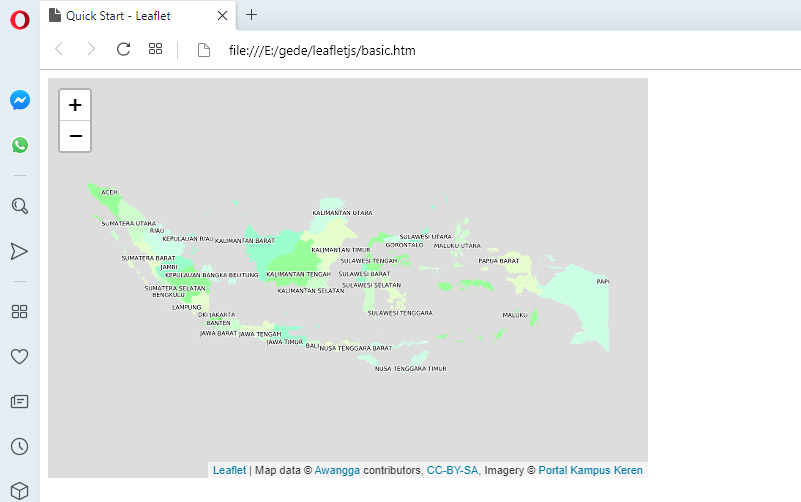
\includegraphics[width=4cm]{figures/tugas4/1174054/3.png}
		\centering
		\caption{File yang telah didownload}
    \end{figure}
    \hfill\break
    \item Selanjutnya, pilih Agree untuk melanjutkan proses instalasi. 
    \hfill\break
    \begin{figure}[H]
		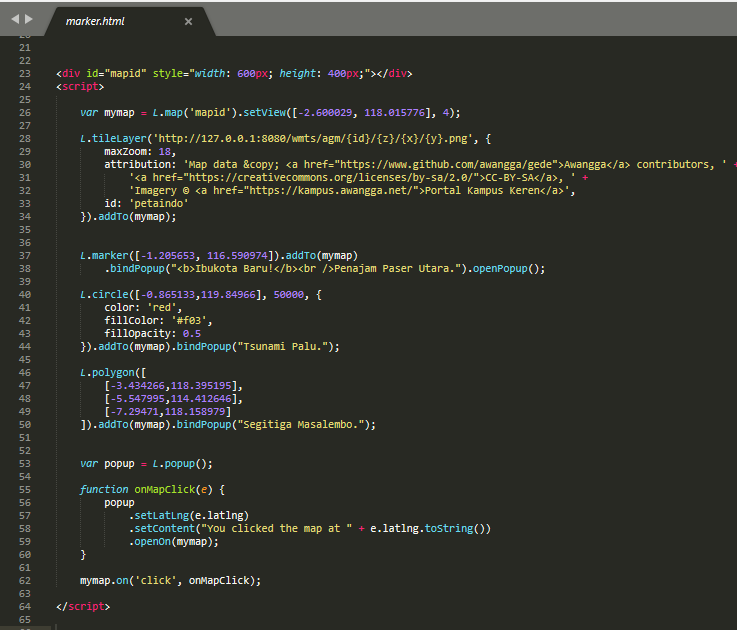
\includegraphics[width=4cm]{figures/tugas4/1174054/4.png}
		\centering
		\caption{Agree Instalasi}
    \end{figure}
    \item Kemudian, pilih Full untuk mendownload full map servernya.
    \hfill\break
    \begin{figure}[H]
		
\includegraphics[width=4cm]{figures/tugas4/1174054/5.png}
		\centering
		\caption{Full Instalasi}
    \end{figure}
    \item Selanjutnya, pilih tempat penyimpanan untuk map servernya, kita bisa menyimpan nya di C
    \hfill\break
    \begin{figure}[H]
		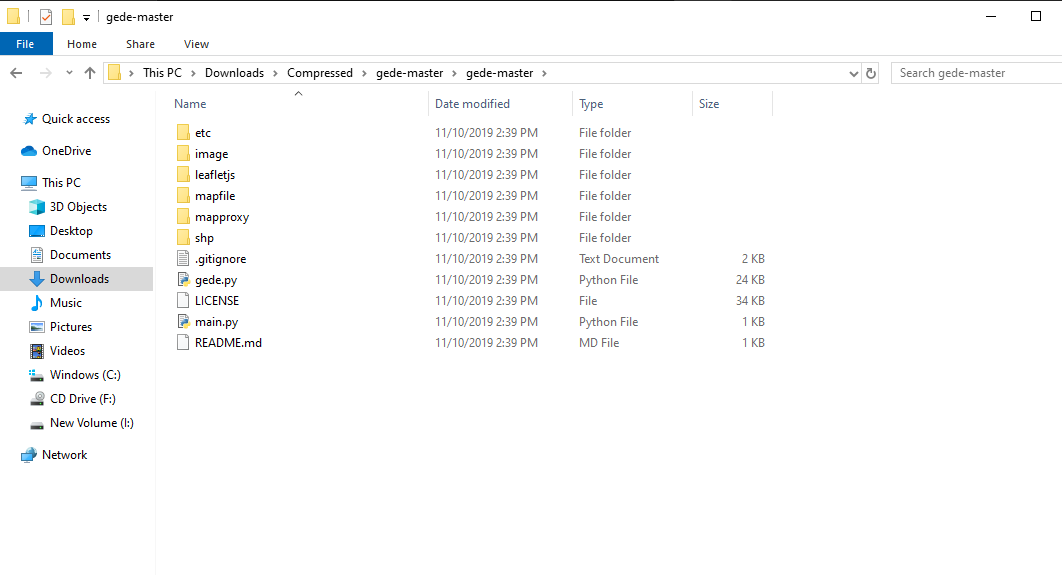
\includegraphics[width=4cm]{figures/tugas4/1174054/6.png}
		\centering
		\caption{Penyimpanan Instalasi}
    \end{figure}
    \item Setelah itu, kita akan menggunakan port 80
    \hfill\break
    \begin{figure}[H]
		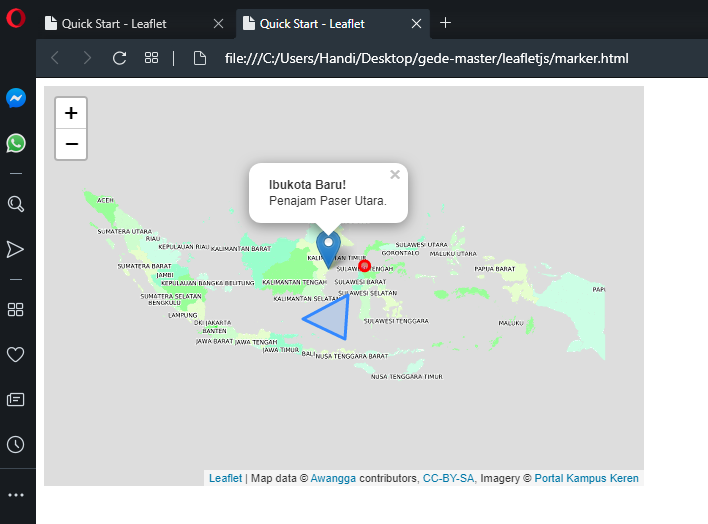
\includegraphics[width=4cm]{figures/tugas4/1174054/7.png}
		\centering
		\caption{Menggunakan Port 80}
    \end{figure}
    \item Tunggu sampai proses instalasi berakhir.
    \begin{figure}[H]
		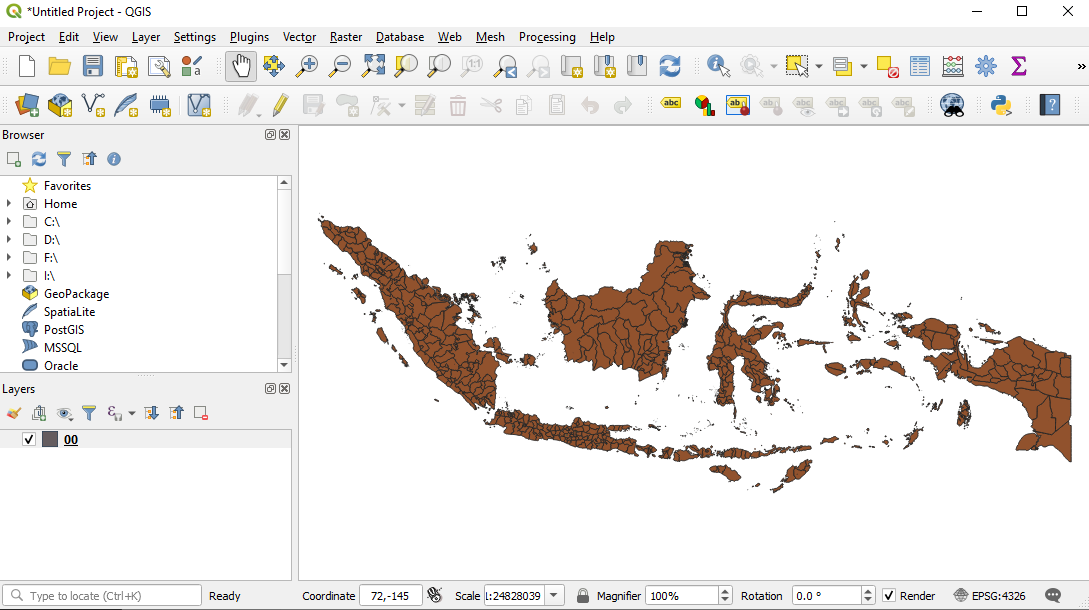
\includegraphics[width=4cm]{figures/tugas4/1174054/8.png}
		\centering
		\caption{Proses Instalasi}
    \end{figure}
    \item Instal vcredist 2017, untuk bisa menjalankan map server. untuk linknya bisa https://support.microsoft.com/id-id/help/2977003/the-latest-supported-visual-c-downloads
\end{enumerate}
\subsection{Konfigurasi Map Server}
Jika telah selesai melakukan instalasi map server kita akan melakukan konfigurasi map server
\begin{enumerate}
  \item Pertama, Buka terlebih dahulu folder ms4w tadi
  \hfill\break
    \begin{figure}[H]
		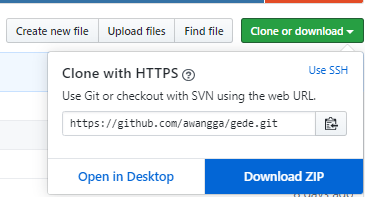
\includegraphics[width=4cm]{figures/tugas4/1174054/9.png}
		\centering
		\caption{Membuka folder ms4w}
    \end{figure}
    \hfill\break
    \begin{figure}[H]
		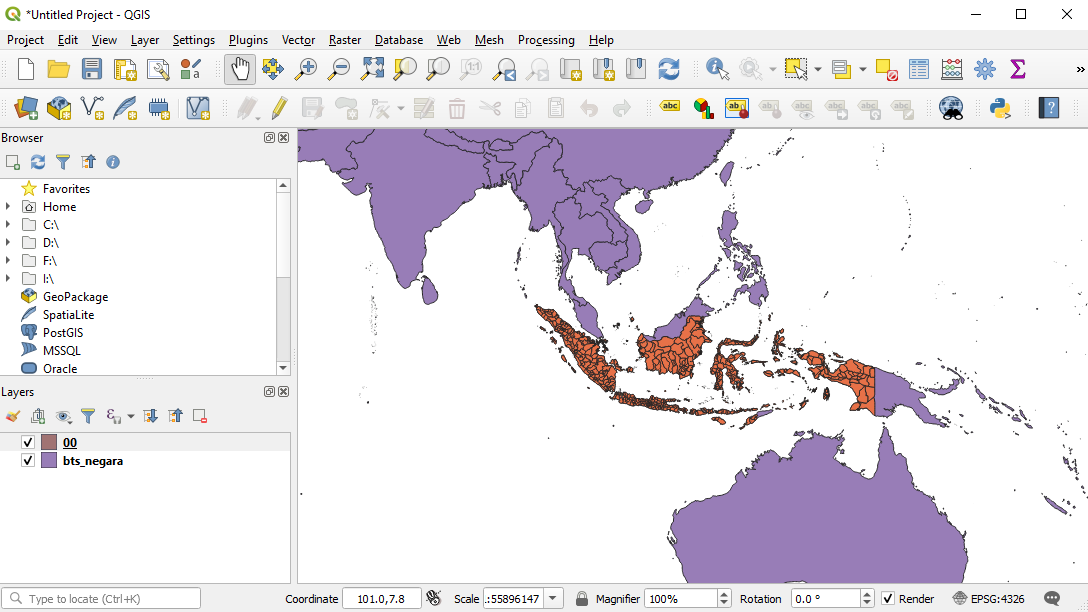
\includegraphics[width=4cm]{figures/tugas4/1174054/10.png}
		\centering
		\caption{Isi Folder ms4w}
    \end{figure}
  \item Selanjutnya, Masuk ke folde apache. Didalam folder apache akan nampak seperti pada gambar berikut:
  \hfill\break
    \begin{figure}[H]
		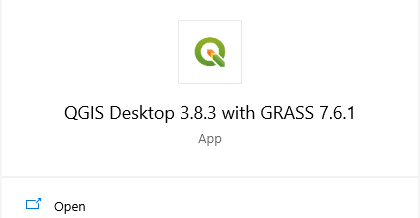
\includegraphics[width=4cm]{figures/tugas4/1174054/11.png}
		\centering
		\caption{Isi Folder Apache}
    \end{figure}
  \item Kemudian, Masuk ke folder conf
  \hfill\break
    \begin{figure}[H]
		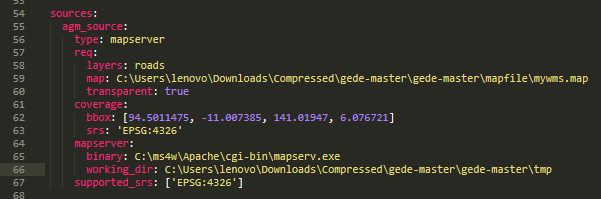
\includegraphics[width=4cm]{figures/tugas4/1174054/12.png}
		\centering
		\caption{Isi Folder Conf}
    \end{figure}
  \item Selanjutnya, Buka file httpd.conf kemudian ubah listen port nya. Karena saya menggunakan port 80 untuk webserver, port ini juga dapat di setting saat proses instalasi sebelumnya.
  \hfill\break
    \begin{figure}[H]
		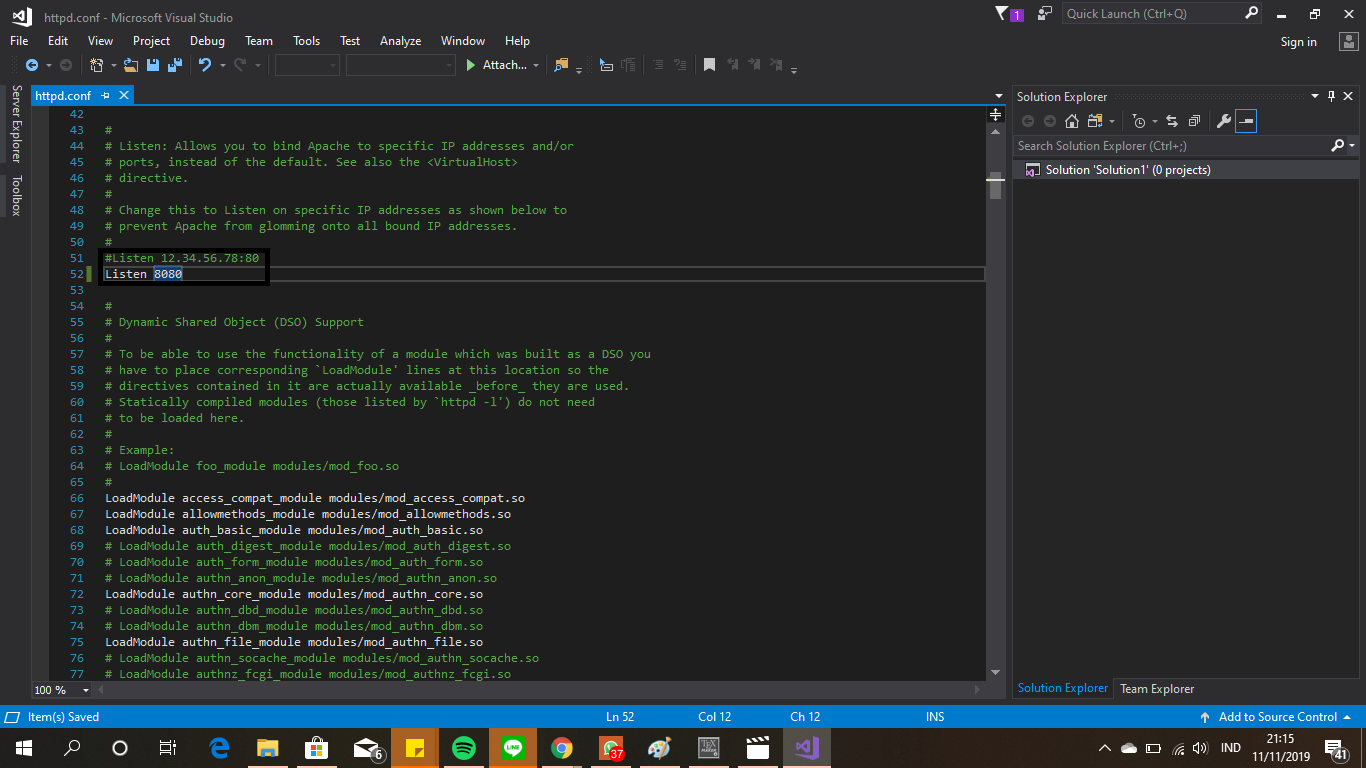
\includegraphics[width=4cm]{figures/tugas4/1174054/13.png}
		\centering
		\caption{Listen port}
    \end{figure}
  \item Kemudian kita jalankan servisnya, dengan menggunakan tombol windows + r dan ketikan services.msc
  \hfill\break
    \begin{figure}[H]
		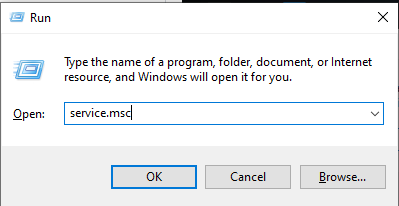
\includegraphics[width=4cm]{figures/tugas4/1174054/14.png}
		\centering
		\caption{Mengakses Halaman Service}
    \end{figure}
  \item Cari servis untuk Apache MS4W Web Server
  \item Jika sudah menemukannya klik 2x
  \item Dan setting seperti berikut
  \hfill\break
    \begin{figure}[H]
		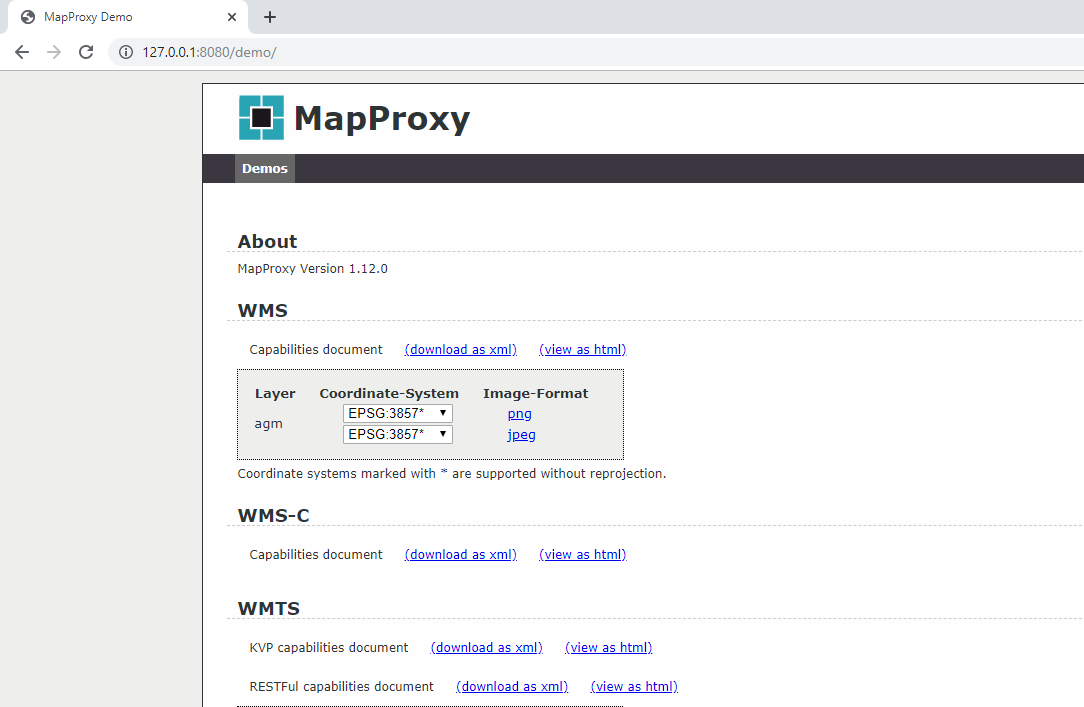
\includegraphics[width=4cm]{figures/tugas4/1174054/15.png}
		\centering
		\caption{Pengaturan Service Apache MS4W Web Server}
    \end{figure}
\end{enumerate}
\subsection{Pengujian}
\begin{enumerate}
  \item Sekarang, Masuklah Ke folder httpd.d yang ada di folder ms4w
  \hfill\break
    \begin{figure}[H]
		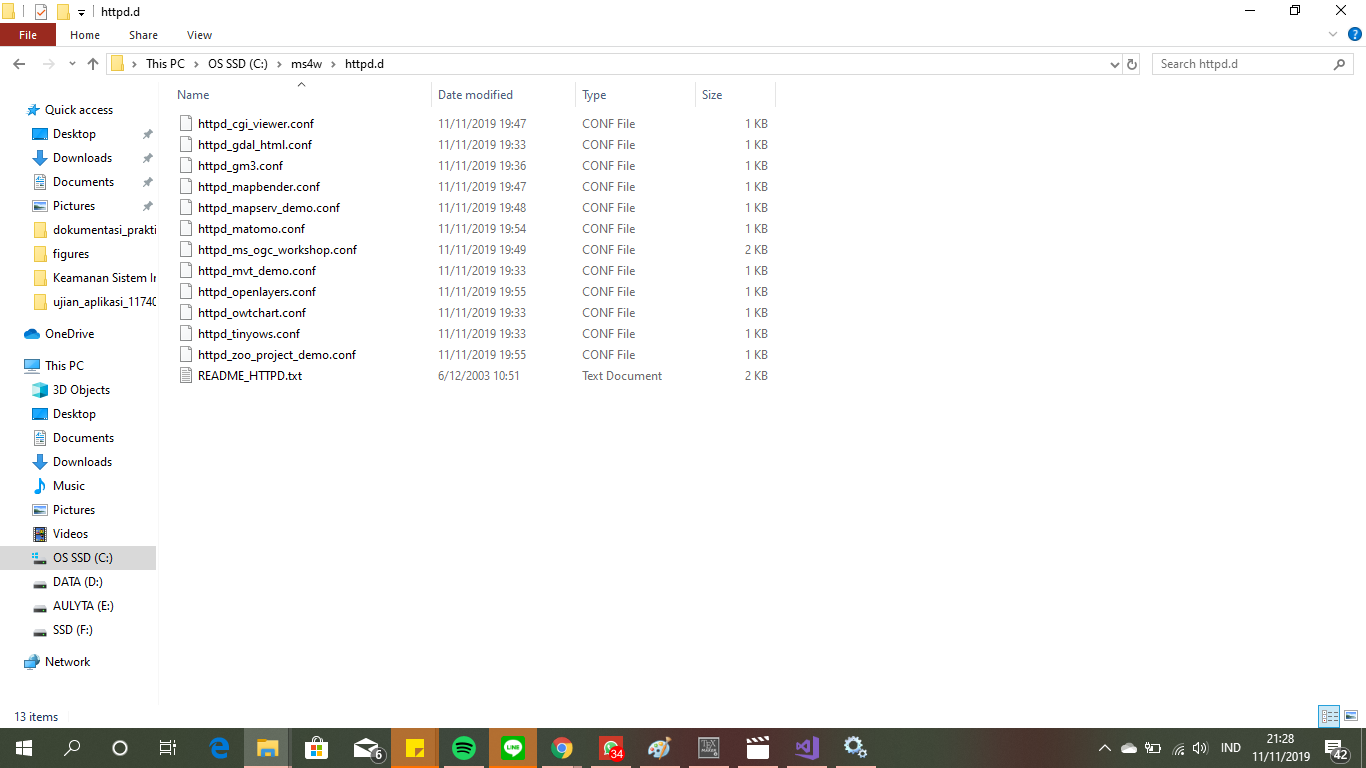
\includegraphics[width=4cm]{figures/tugas4/1174054/16.png}
		\centering
		\caption{Isi Folder httpd.d}
    \end{figure}
  \item Buat sebuah file dengan nama httpd mywfs conf
  \hfill\break
    \begin{figure}[H]
		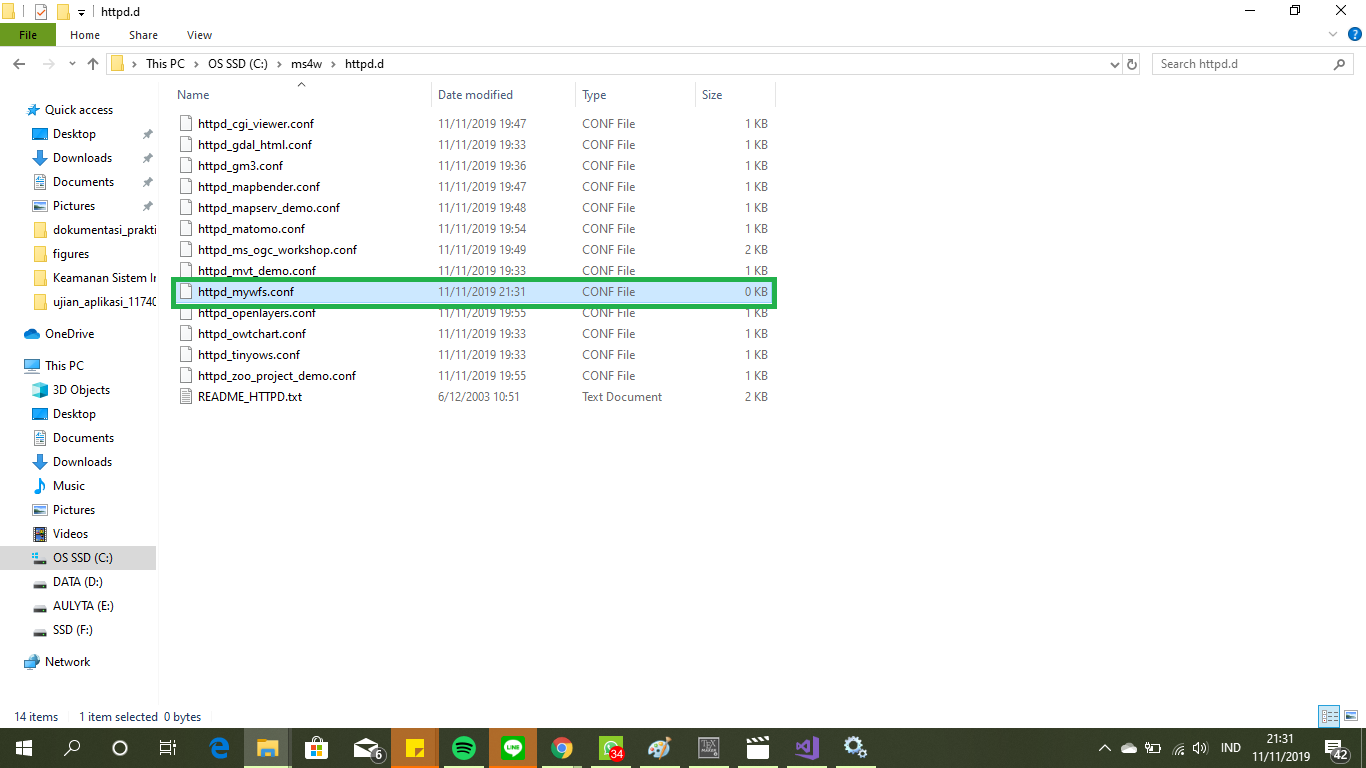
\includegraphics[width=4cm]{figures/tugas4/1174054/17.png}
		\centering
		\caption{Membuat file baru}
    \end{figure}
  \item Buka file httpd mywfs conf yang baru dibuat dan ubah isinya menjadi seperti berikut
  \hfill\break
    \begin{figure}[H]
		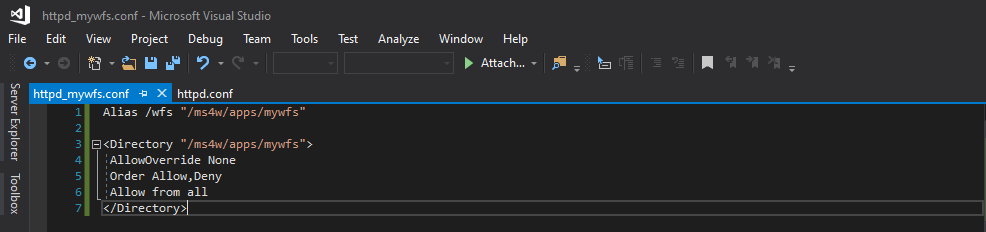
\includegraphics[width=4cm]{figures/tugas4/1174054/18.png}
		\centering
		\caption{Konfigurasi File Tersebut}
    \end{figure}
  \item Buka Folder apps yang ada di folder ms4w
  \hfill\break
    \begin{figure}[H]
		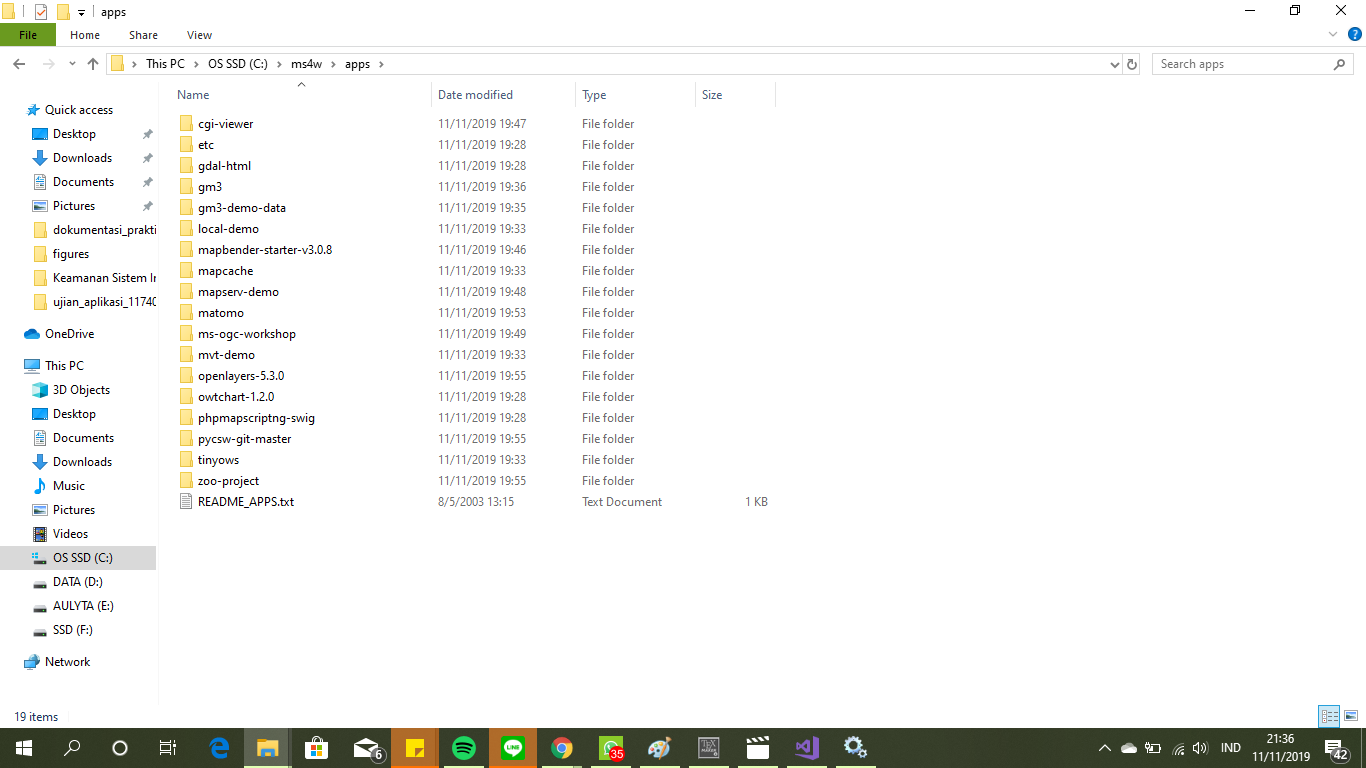
\includegraphics[width=4cm]{figures/tugas4/1174054/19.png}
		\centering
		\caption{Isi Folder Apps}
    \end{figure}
  \item Buat sebuah folder baru disana dengan nama mywfs,karena sebelumnya menyeting di httpd mywfs conf nya seperti itu
  \hfill\break
    \begin{figure}[H]
		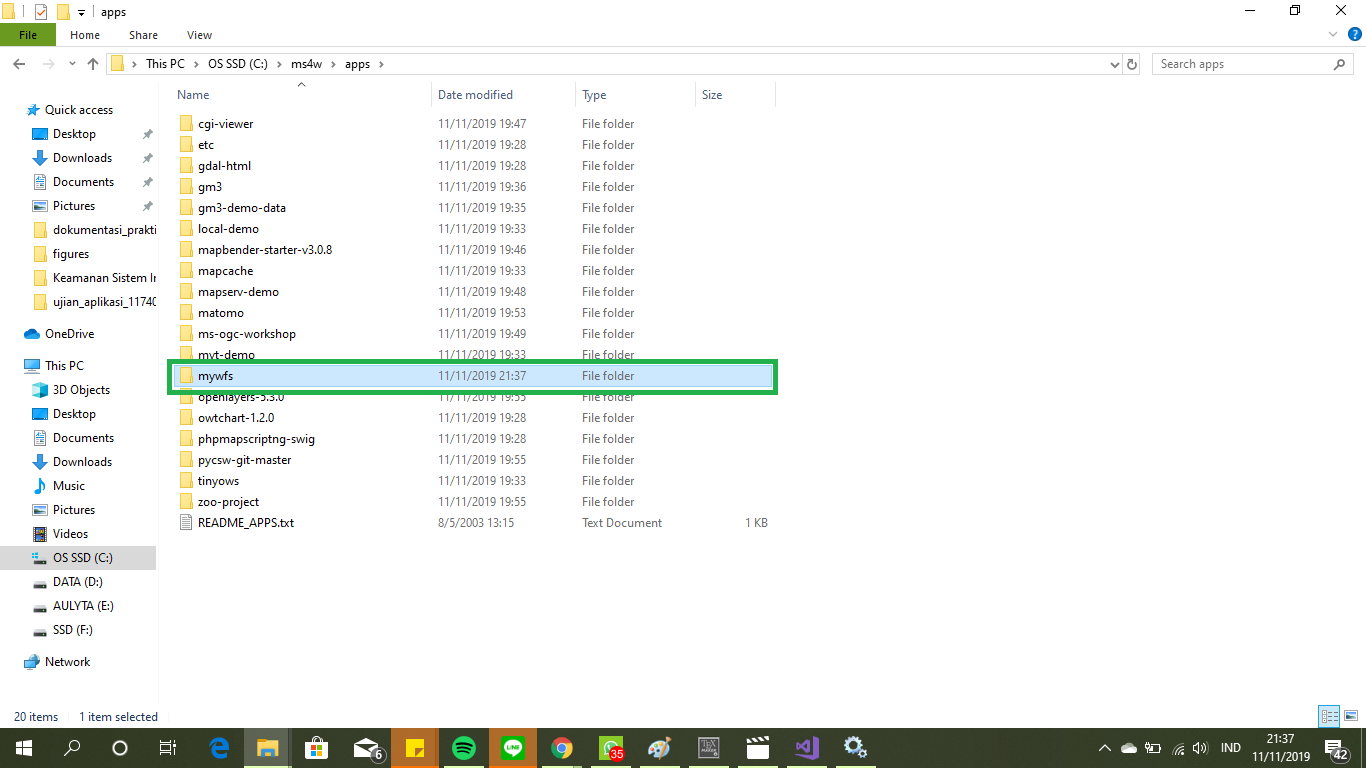
\includegraphics[width=4cm]{figures/tugas4/1174054/20.png}
		\centering
		\caption{Membuat folder baru}
    \end{figure}
  \item Di dalam folder mywfs buat file baru dengan nama mywfs.map
  \hfill\break
    \begin{figure}[H]
		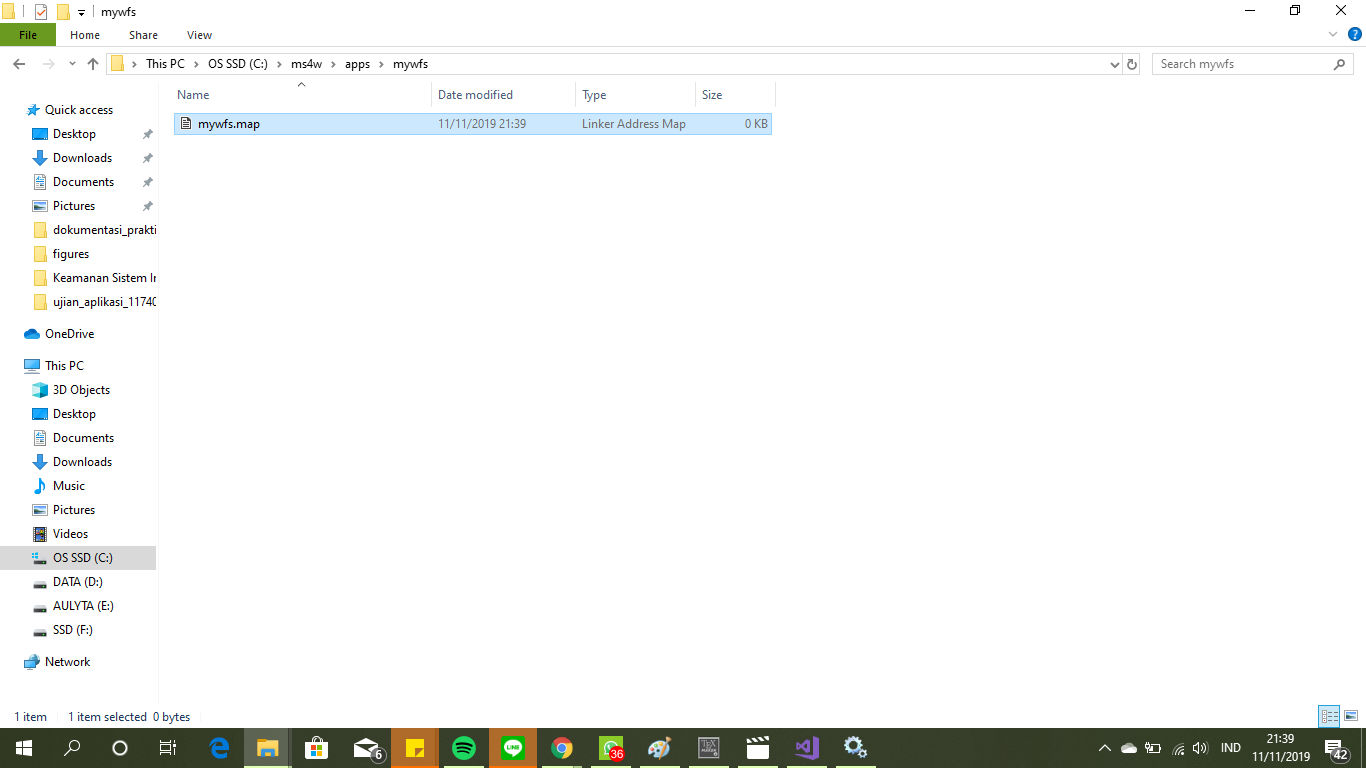
\includegraphics[width=4cm]{figures/tugas4/1174054/21.png}
		\centering
		\caption{Membuat file baru}
    \end{figure}
  \item Modifikasi isinya menjadi sebagai berikut
  \hfill\break
    \begin{figure}[H]
		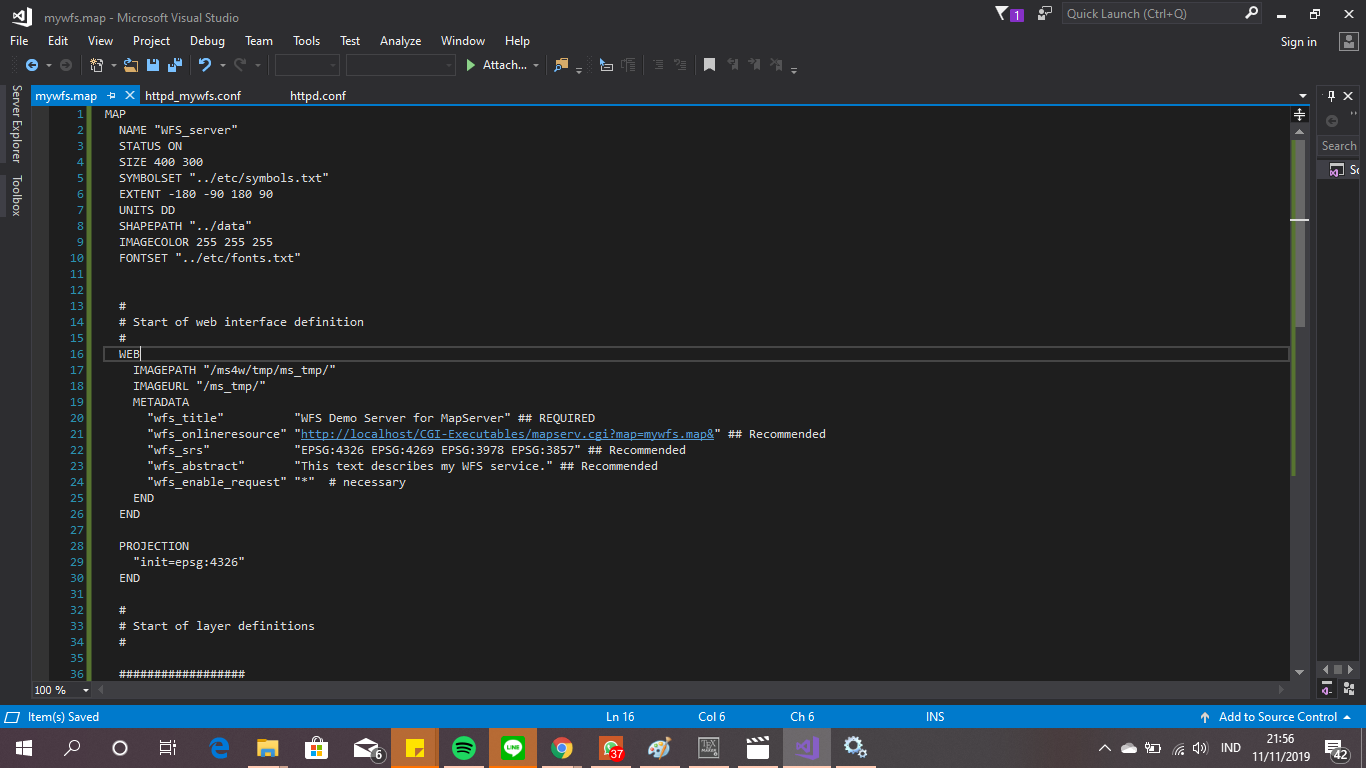
\includegraphics[width=4cm]{figures/tugas4/1174054/22.png}
		\centering
		\caption{Isi mywfs.map 1}
    \end{figure}
    \hfill\break
    \begin{figure}[H]
		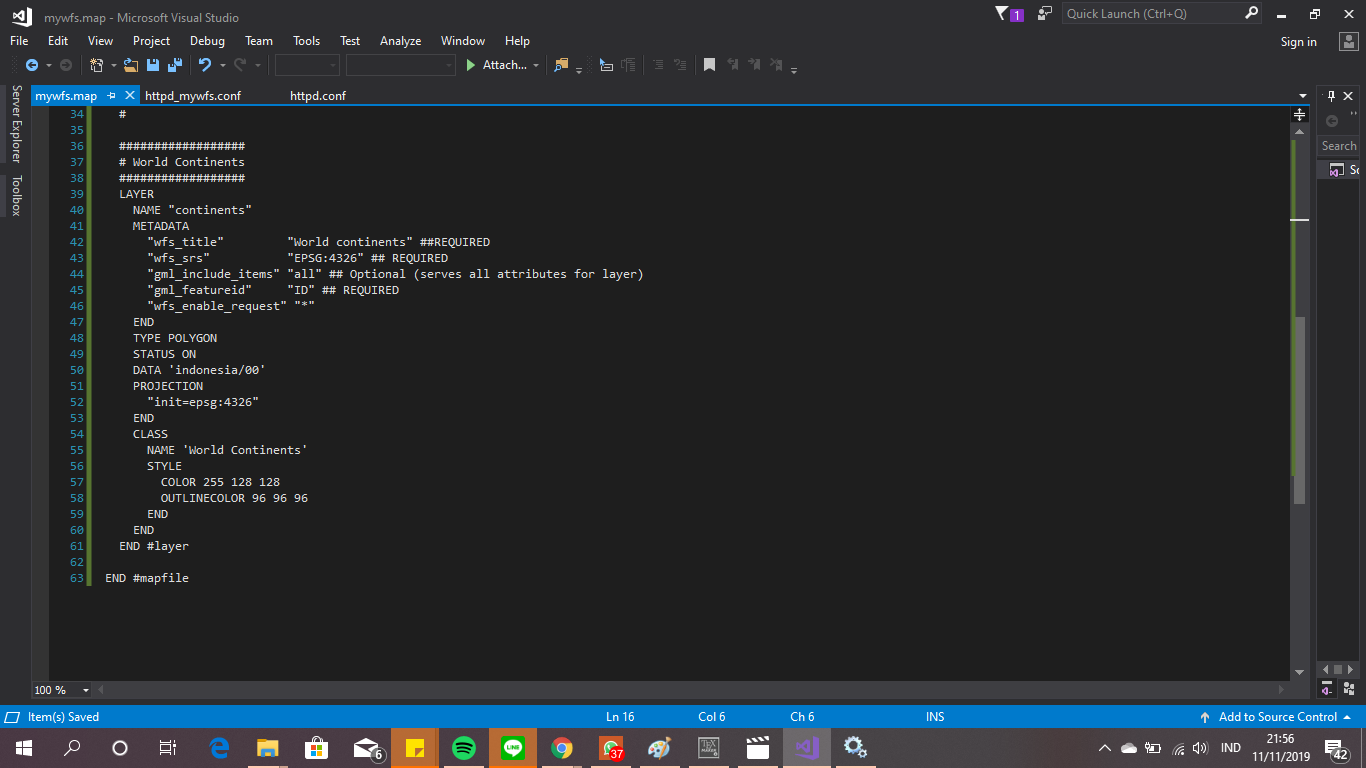
\includegraphics[width=4cm]{figures/tugas4/1174054/23.png}
		\centering
		\caption{Isi mywfs.map 2}
    \end{figure}
  \item Dan sekarang buka file .shp nya, dan lihat hasil nya
  \hfill\break
  \begin{figure}[H]
  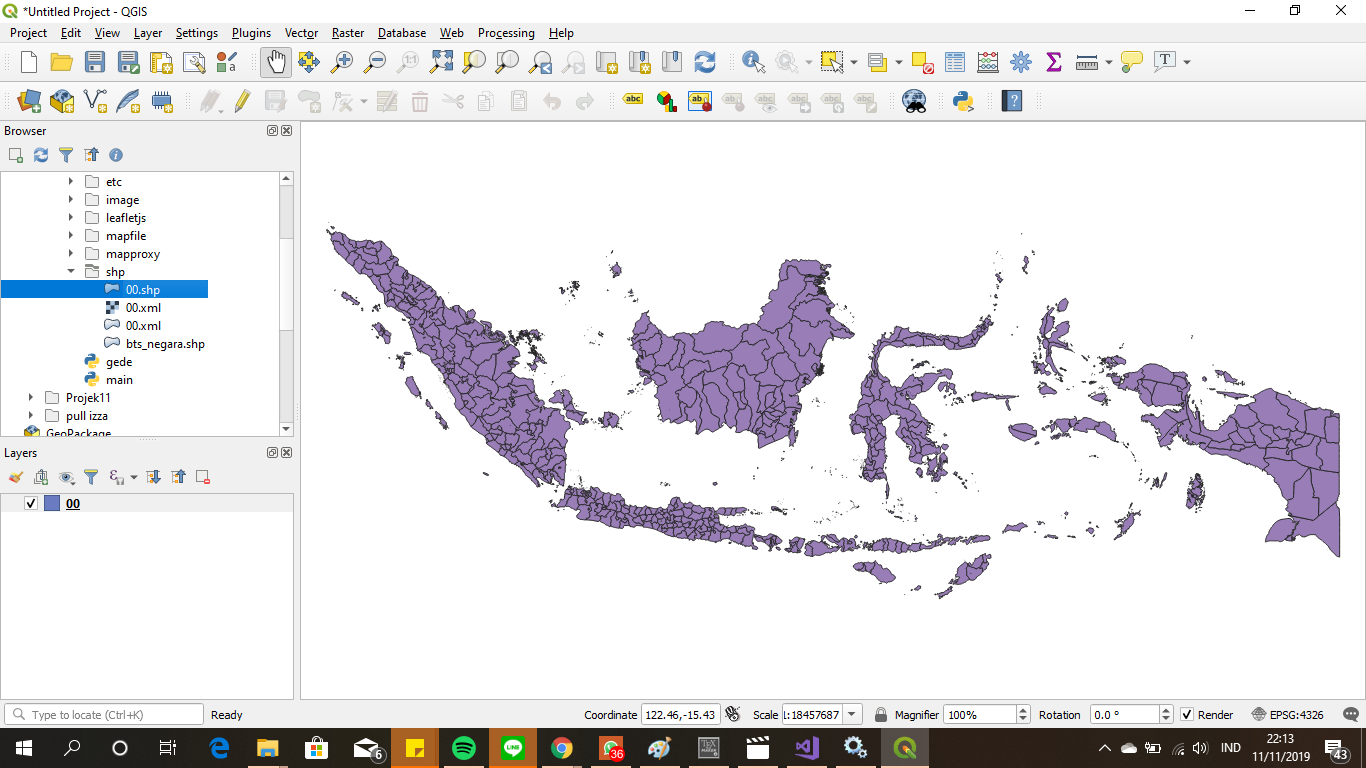
\includegraphics[width=4cm]{figures/tugas4/1174054/24.png}
  \centering
  \caption{Hasil}
  \end{figure}
\end{enumerate}
\subsection{Link Youtube}
https://youtu.be/woKB9MKO3G4
\subsection{Instalasi Map Proxy}
\begin{enumerate}
  \item Pertama, Buka Command Prompt/cmd pada Windows
  \item Kemudian ketik pip install MapProxy, seperti pada gambar berikut :
  \hfill\break
  \begin{figure}[H]
  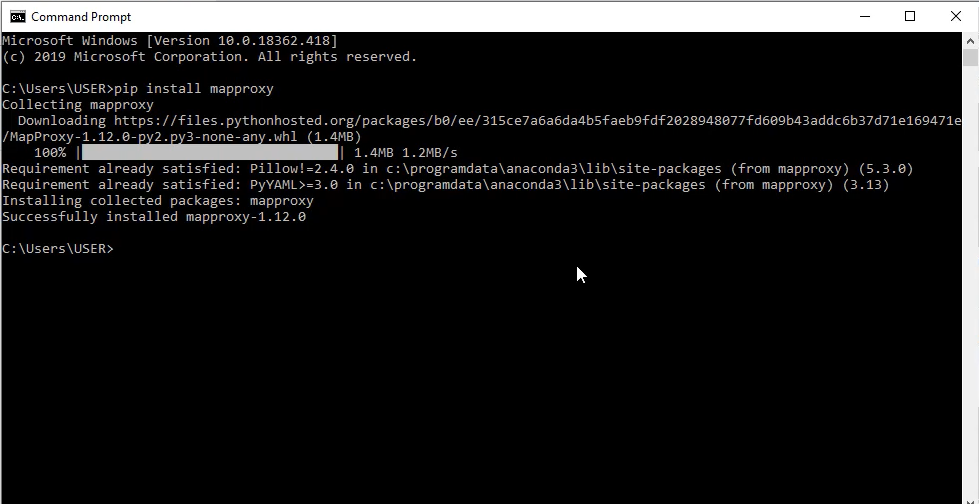
\includegraphics[width=4cm]{figures/tugas4/1174054/25.png}
  \centering
  \caption{Instalasi MapProxy}
  \end{figure}
\end{enumerate}
\subsection{Membuka Map menggunakan MapProxy}
\begin{enumerate}
  \item Pertama,Download atau clone git dari https://github.com/awangga/gede
  \item Pastikan path menuju folder gede tidak ada spasi contohnya saya F:/gede-master
  \item Pada folder gede-master buat folder bernama tmp
  \hfill\break
  \begin{figure}[H]
  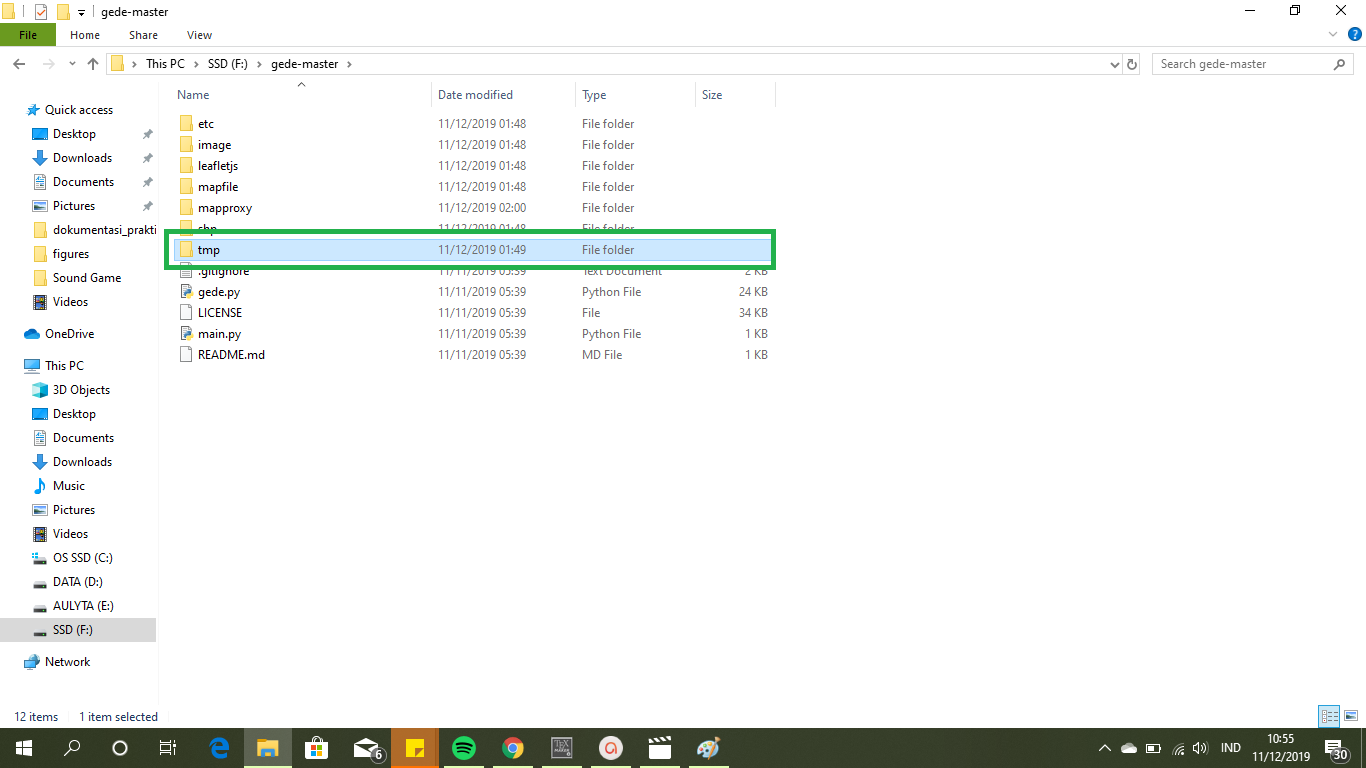
\includegraphics[width=4cm]{figures/tugas4/1174054/26.png}
  \centering
  \caption{Buat folder tmp}
  \end{figure}
  \item Setelah itu buka folder mapproxy lalu edit file agm.yaml
  \item Edit pada bagian sources lalu ada map, masukkan pathnya sesuai dengan dimana anda menyimpan file gede yang anda clone contohnya saya ada pada F:/gede-master/mapfile/mywms.map
  \hfill\break
  \begin{figure}[H]
  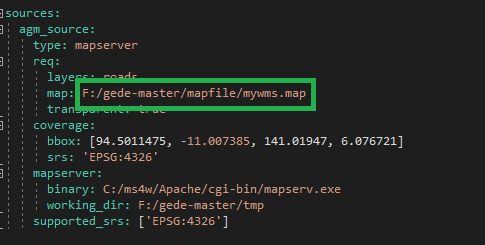
\includegraphics[width=4cm]{figures/tugas4/1174054/27.png}
  \centering
  \caption{Edit lokasi mymap.map}
  \end{figure}
  \item Lalu dibawahnya pada bagian binary masukkan lokasi instalasi ms4w anda, lalu tambahkan /Apache/cgi-bin/mapserv.exe, yang saya setelah diedit menjadi C:/ms4w/Apache/cgi-bin/mapserv.exe
  \hfill\break
  \begin{figure}[H]
  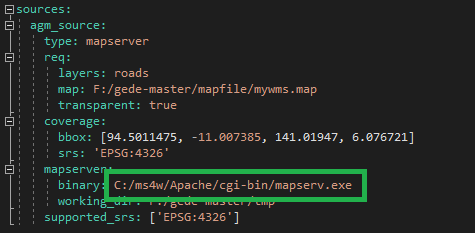
\includegraphics[width=4cm]{figures/tugas4/1174054/28.png}
  \centering
  \caption{Edit path binary mapserv}
  \end{figure}

  \item Setelah itu pada bagian working-dir masukkan path folder yang telah kita buat tadi, yang saya F:/gede-master/tmp
  \hfill\break
  \begin{figure}[H]
  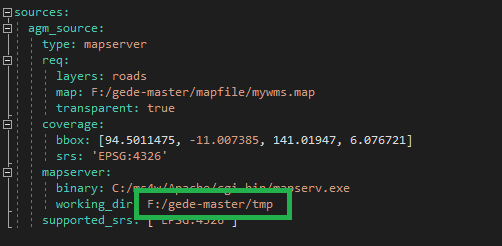
\includegraphics[width=4cm]{figures/tugas4/1174054/29.png}
  \centering
  \caption{Edit path working-dir}
  \end{figure}

  \item Setelah itu buka aplikasi MS4W-Shell

  \item Setelah itu buka lokasi folder gede kita yang tadi telah di clone dan buka juga folder mapproxy yang ada pada folder gede
  \hfill\break
  \begin{figure}[H]
  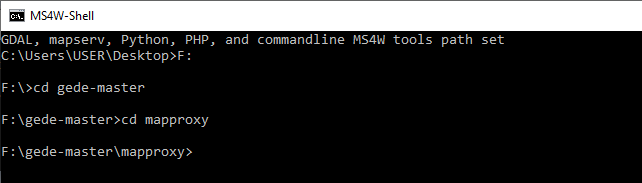
\includegraphics[width=4cm]{figures/tugas4/1174054/30.png}
  \centering
  \caption{Buka Folder gede dan mapproxy}
  \end{figure}

  \item setelah dibuka ketikkan "mapproxy-util serve-develop ./agm.yaml" pada ms4w-Shell untuk membuka aplikasi mapproxy
  \hfill\break
  \begin{figure}[H]
  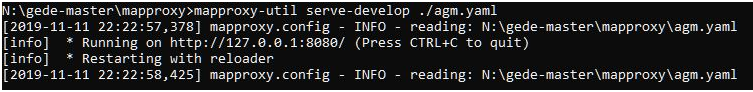
\includegraphics[width=4cm]{figures/tugas4/1174054/31.png}
  \centering
  \caption{Buka aplikasi mapproxy}
  \end{figure}
  
  \item Buka browser lalu ketikkan 127.0.0.1:8080
  \hfill\break
  \begin{figure}[H]
  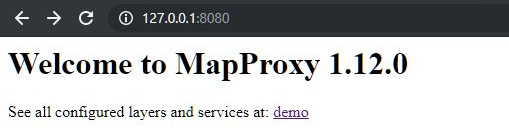
\includegraphics[width=4cm]{figures/tugas4/1174054/32.png}
  \centering
  \caption{Buka mapproxy pada browser}
  \end{figure}

  \item lalu klik demo untuk melihat map
  \item lalu klik png pada agm, maka mapproxy akan menampilkan map
  \hfill\break
  \begin{figure}[H]
  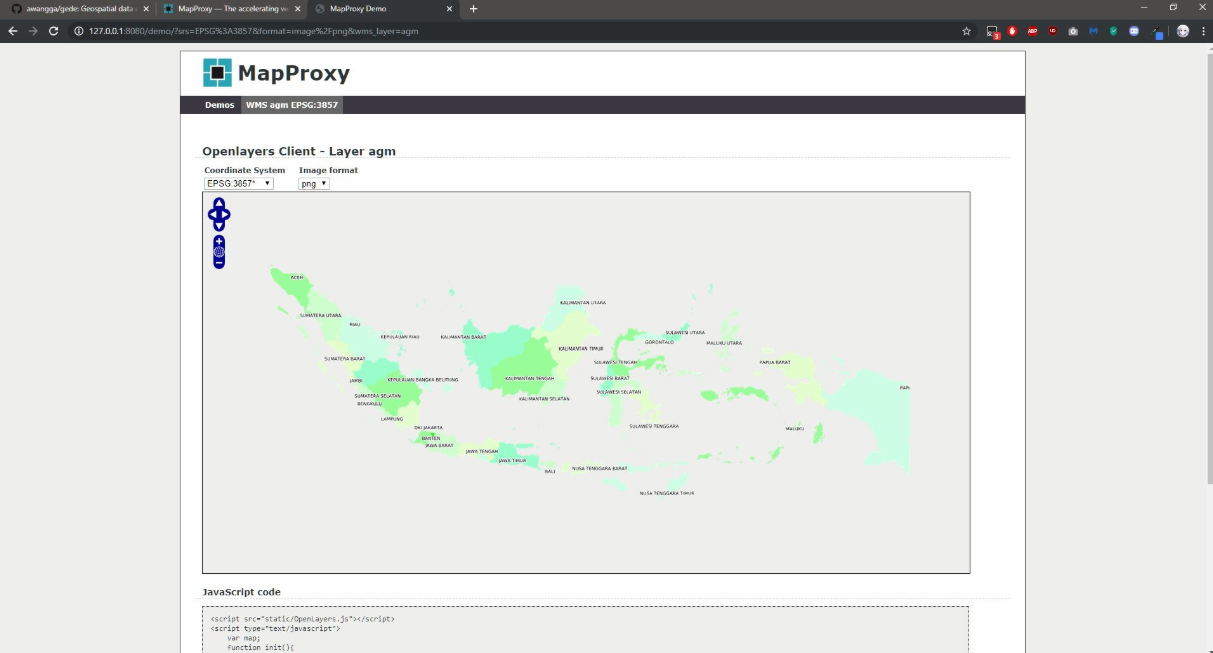
\includegraphics[width=4cm]{figures/tugas4/1174054/33.png}
  \centering
  \caption{MapProxy menampilkan map}
  \end{figure}

\end{enumerate}
\subsection{Link Youtube MapProxy}
https://youtu.be/CAt1ceT0W9Y